\documentclass{article}

\usepackage[utf8]{inputenc}
\usepackage[T1]{fontenc}

\usepackage{Sweave}
\begin{document}
\Sconcordance{concordance:perceptron_simples.tex:perceptron_simples.Rnw:%
1 5 1 1 0 12 1 1 2 1 0 1 2 1 1 2 2 1 1 1 2 2 1 1 2 1 1 1 2 1 1 4 0 1 2 %
4 1 1 3 1 0 1 2 1 1 2 2 1 1 1 9 7 0 1 2 5 0 1 3 1 1}


\title{Perceptron Simples}
\author{Matheus Araujo - 2013066265}
\date{}

\maketitle

\section{Amostragem}

A seguir é apresentado o código que gera as duas distribuições, $\texttt{xc1} = \mathcal{N}(2,2,\sigma^2)$ $\texttt{xc2} = \mathcal{N}(4,4,\sigma^2)$ e também a reta $x_2 = -x_1+6$.

\begin{Schunk}
\begin{Sinput}
>   rm(list = ls())
>   xc1<-matrix(rnorm(100,sd=0.4),ncol=2)+2
>   xc2<-matrix(rnorm(100,sd=0.4),ncol=2)+4
>   plot(xc1[,1],xc1[,2],col='red',xlim=c(0,6),ylim=c(0,6),xlab='',ylab='')
>   par(new=T)
>   plot(xc2[,1],xc2[,2],col='blue',xlim=c(0,6),ylim=c(0,6),xlab='',ylab='')
>   w1<-1
>   w2<-1
>   theta<-6
>   fx1<-seq(0,6,0.1);
>   fx2<--w1/w2*fx1+theta/w2
>   par(new=T)
>   plot(fx1,fx2,col='black',type='l')
\end{Sinput}
\end{Schunk}
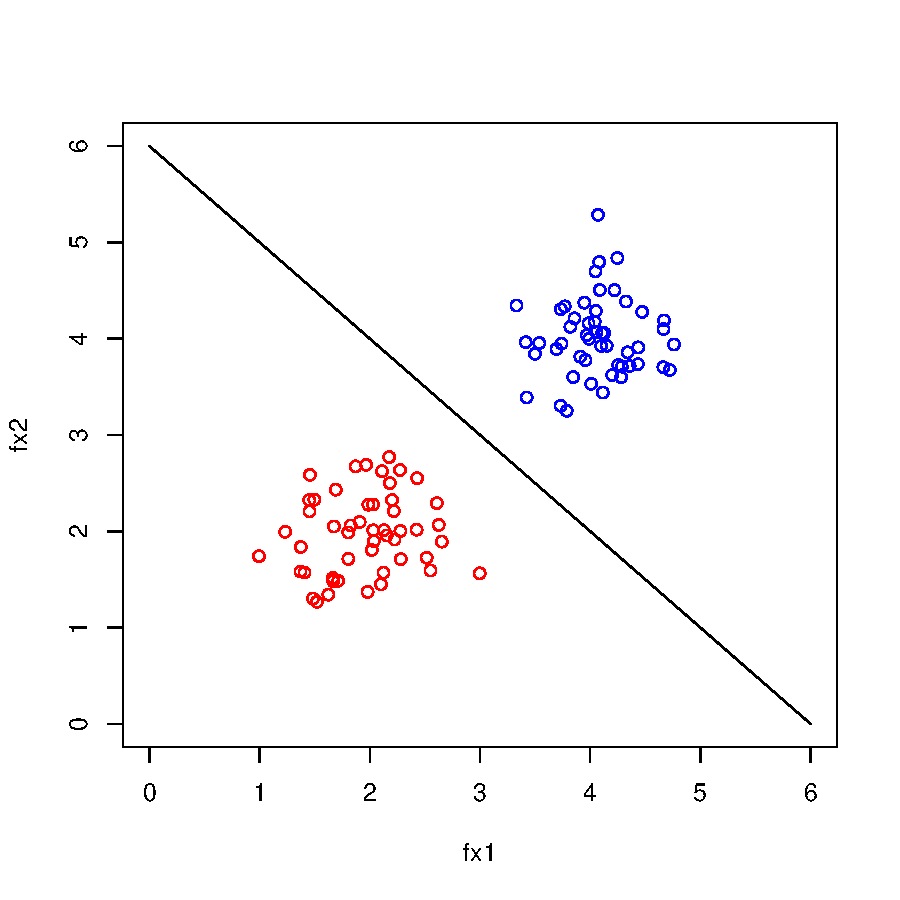
\includegraphics{perceptron_simples-001}

\section{Perceptron Simples}

O código mostrado a seguir é o para o \textit{Perceptron Simples}.

\begin{Schunk}
\begin{Sinput}
>   library('plot3D')
>   seqi<-seq(0,6,0.1)
>   seqj<-seq(0,6,0.1)
>   M<-matrix(1,nrow=length(seqi),ncol=length(seqj))
>   ci<-0
>   cj<-0
>   for(i in seqi) {
+     ci<-ci+1
+     cj<-0
+     for(j in seqj) {
+       cj<-cj+1
+       M[ci,cj]<-1*(i*w1+j*w2>=theta)
+     }
+   }
>   persp3D(seqi,seqj,M)
>   
\end{Sinput}
\end{Schunk}
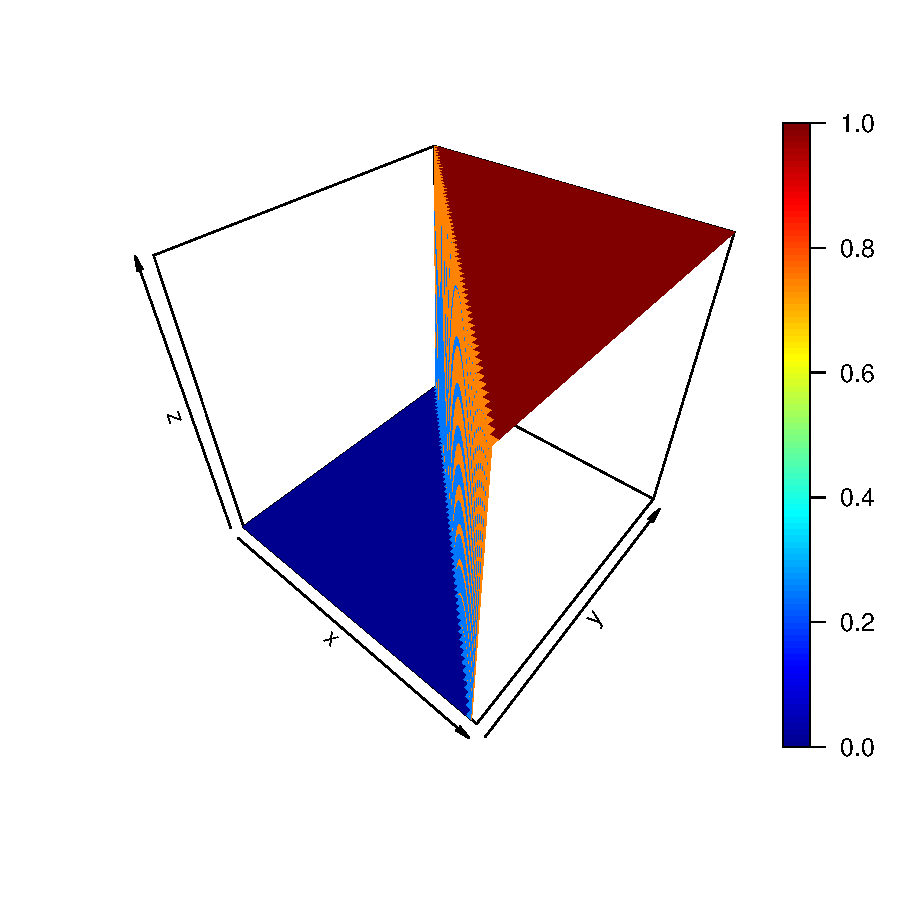
\includegraphics{perceptron_simples-002}

\end{document}
